In this chapter, we describe the approach which we have adopted to create the dynamic benchmark of executable python software. The overall workflow of the approach is shown in the Figure \ref{fig:overall_approach}.

With the provided approach, our benchmark aims to achieve the properties of being large-scale, diverse, ready to run, ready to analyze, compositional and long term. We start with a large corpus of open source python projects listed in the awesome-python project (Section \ref{approach:corpus of python projects}). The projects are selected from this large corpus based on the selection criteria as described in Section \ref{approach:selection criteria}. This selection gives us a collection of python projects in the form of GitHub URLs and certain flags in a text file (Section \ref{approach:list of projects}). Bash scripts use this collection of projects in order to automate the installation of projects and their dependencies (Section \ref{approach:bash scripts}) which provides a set of installed python projects and the environment for use by developers and researchers as described in Section \ref{approach:collection of projects}. With the help of a python script (Section \ref{approach:python script}), a single command line interface provides easy access to the benchmark which consists of the installed projects along with various analysis tools and frameworks (Section \ref{approach:command line interface}). The benchmark containing the installed projects along with its command line interface is packaged and exported as a docker container for use by researchers and developers (Section \ref{approach: packing and exporting}). The command line interface incorporates  analysis frameworks like LExecutor, DynaPyt and PyCG into the benchmark for execution of various tasks such as dynamic analysis, trace file generation, and static call graph generation respectively (Section \ref{approach:analysis framework}).

\begin{figure}[ht]
\centering
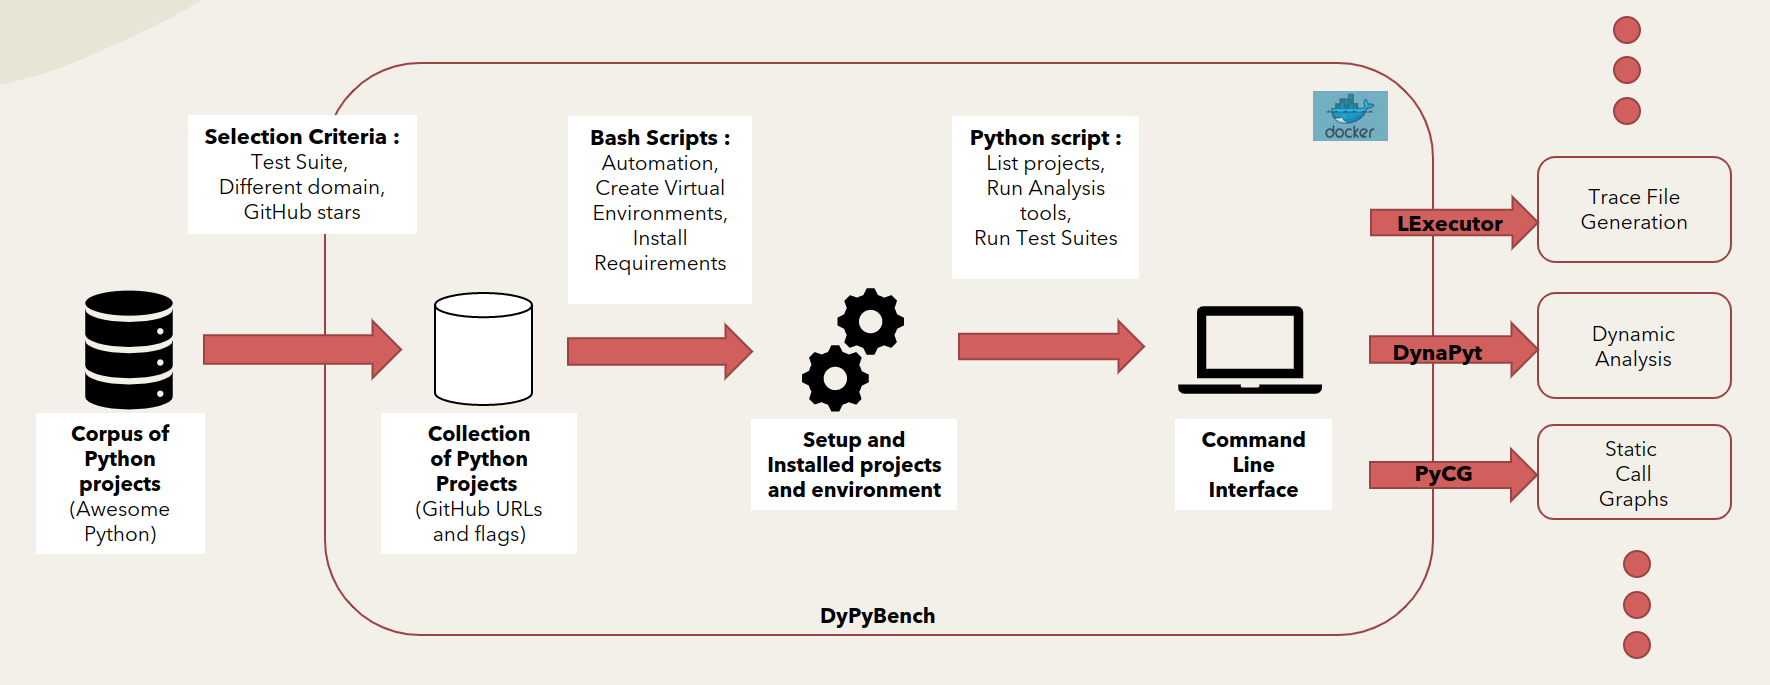
\includegraphics[width=1\linewidth]{figures/approach/DyPyBench.png}
\caption[Approach]{\label{fig:overall_approach}Overall Approach of DyPyBench.}
\end{figure}

\section{Corpus of Python projects}
\label{approach:corpus of python projects}
Python's ease of use and popularity, as well as the usage in different domains has led to a large number of projects being developed and made available to the community as open source software. GitHub alone contains more than 510000 public repositories that have python as their primary programming language \cite{bing_chat}(Bing Chat??). However, GitHub does not state which of these projects belong to which application domain. Also, it is difficult to go through 51000 repositories to filter out the projects from different domains without any classification.
This classification issue is solved with the help of Awesome-Python project, which is an open source project available on GitHub. This project contains a list of some of the most useful and interesting open source python projects including libraries, frameworks and software. Additionally, the awesome-python project classifies the python projects based on different categories which in essence represent the application domain of the project.
The awesome-python project acts as a corpus for our benchmark as it provides 679 python projects. It further classifies these projects into 92 main categories, out of which some of the categories can be further divided into sub-categories. Some of the categories and the number of projects in those are listed in table \ref{table:awesome-python}. For more details on the various categories and number of projects in each provided by the awesome-python project refer to the appendix \ref{appendix:awesome python projects}.

\begin{table}[ht]
    \centering
    \begin{tabular}{lc}
    \hline
    \textbf{Category} & \textbf{Number of Projects}\\
    \hline
    Admin Panels    & 9\\
    Code analysis   & 18\\
    Computer vision & 7\\
    Deep Learning   & 7\\
    Documentation   & 3\\
    Files   & 7\\
    GUI development & 16\\
    Robotics    & 2\\
    Task Queues & 5\\
    Web Frameworks  & 5\\
    \hline
    \end{tabular}
    \caption{Project Categories (Awesome Python)}
    \label{table:awesome-python}
\end{table}

\section{Selection Criteria}
\label{approach:selection criteria}
The corpus of python projects provides us with a large number of python projects to choose from diverse application domains. However, the benchmark must contain a restricted number of projects which fulfill the requirements that can make benchmark useful for its intended purpose. The selection criteria does exactly this for our benchmark, i.e., it makes our benchmark large scale and diverse by selecting 50 python projects from the available corpus. The selection criteria of diverse domain ensures that we select the projects which belong to different categories as described in the section \ref{approach:corpus of python projects}. The count of 50 projects ensures that we have sufficiently large number of projects in the benchmark for usage by different analysis tools. Since, in this work we are creating a dynamic benchmark we focus on the projects for which we can perform execution. Test suites provide us with a files which can be easily execute the code using testing libraries such as pytest, unittest, flake8, etc. As a result we include the criterion of presence of test suites for the selection process. However, we limit the execution of tests via pytest as it is a popular testing library and is also used by the DynaPyt framework used for analysis. The number of stars a project has on GitHub is be an indication of how popular and well-regarded it is in the community. More stars generally mean more people have found the project useful and interesting, and it has a larger user base and community of contributors. Since a benchmark must contain useful and meaningful projects, we include the criterion of a minimum 500 GitHub stars for the project selection. This is also a common practice among benchmarks in other languages such as Java Microbenchmark Harness (JMH), and Google Benchmark. 

\section{List of Python Projects}
\label{approach:list of projects}
Applying the selection criteria as described in section \ref{approach:selection criteria} we obtain a list of 50 open-source python projects from diverse application domains. Since, the projects have their own installation dependencies and source code structure, we need a generic way to handle the setup, installation and execution of these projects within the benchmark. In this work, we handle such details by the means of a text file that contains the GitHub URL, flag and test details for each of the 50 projects. Each line in this collection text file has the details of one project in the benchmark. The GitHub URL helps us in obtaining the source code of the project needed by the analysis tools and frameworks. The flag indicates the presence or absence of requirements file in order to install dependencies for the project. If this flag specifies the presence of the requirement file then the collection text file also contains the path of the requirements file. The need for the path arises due the different structure of source code for individual projects. The collection text file also specifies the path of the test directory or the test file to be run using the pytest library. The table \ref{table:list of projects} shows the structure of the collection text file containing the list of 50 python projects in the benchmark. The first row indicates the entry with the presence of requirements file, while the second row indicates the entry with its absence.

\begin{table}[ht]
    \centering
    \begin{tabular}{llll}
    % \hline
    % \textbf{GitHub URL} & \textbf{Flag} & \textbf{Requirement File} & \textbf{Test Path}\\
    \hline
    https://github.com/test/test-project.git    & rt    & src/requirement.txt   & src/tests\\
    https://github.com/test/test-project.git    & t    & src/tests\\
    \hline
    \end{tabular}
    \caption{List of Projects (Collection Text File Structure)}
    \label{table:list of projects}
\end{table}

\section{Bash Scripts}
\label{approach:bash scripts}
With a list of 50 python projects as described in section \ref{approach:list of projects} we get a list of GitHub URLS and flags helpful in setup and installation of individual projects. In order to install and setup these projects for use in the benchmark, there are a number of steps performed for each project as listed below:
\begin{itemize}
    \item \textbf{Get the source code :} The list contains open source projects having their source code on GitHub which is cloned to a specific folder in the benchmark. 
    \item \textbf{Create virtual environment :} The virtualenv \cite{virtualenv} package creates a virtual environment which avoid dependency conflicts and system pollution, dodge installation lockups and minimize reproducibility issues \cite{Why_Virtual_Env}.
    \item \textbf{Install project and its dependencies :} The pip package manager \cite{pip_package_manager} installs the project and its module dependencies from the requirements.txt file or the setup.py file.
\end{itemize}
Manually performing these steps for each of the 50 projects is a mundane task which can be automated using bash scripts. Bash scripts can specify specific commands to run in a sequential order as required for the installation and setup. Bash scripts can also handle repetition and exceptions with loops and conditionals respectively. In this work, a bash script performs the task of cloning the repository, creating virtual environment and installing the project with its dependencies for each of the 50 projects from the list. There are many other bash scripts present in this work that help in automation of various tasks and can be run directly from the command line or from the python script as described in the section \ref{approach:python script}. One of these tasks is installation and updation of the analysis frameworks described in section \ref{approach:analysis framework}. Another task handled by the bash scripts is the execution of the test suites and analysis frameworks.

\section{Collection of Python Projects}
\label{approach:collection of projects}
Executing the bash scripts as described in the section \ref{approach:bash scripts} we obtain a set of 50 python projects which are installed and ready to use in the benchmark. These 50 projects form the collection of projects on which we can perform the analysis using the tools like DynaPyt, LExecutor and PyCG. The collection is present in a folder which further contains numbered folders for each project for ease of use. Each project has its dependencies installed within its own python virtual environment that also contains pytest and any other dependency required to run the test suite of the project without any further assistance. A copy of the specific project from the collection is created whenever we need to perform the analysis. This ensures the long term usage of the benchmark, as the projects preserve their source code and dependencies in the original folder which can change due to the nature of python and open source ecosystem. The collection also ensures that the projects are ready to use and do not require installation every time a project needs to be utilized.

\section{Selected Python Projects}
\label{approach:selection of projects}
Since Python is a very popular and general purpose programming language, it has been used in many domains and we have a large set of open source python projects available on the internet. In this thesis we target projects from many of these varied domains which are well accepted in the community and at the same time open sourced. Another important factor is the availability of test suites in the project source code. 

\section{Setup and Install}
\label{approach:setup and install}
With a set of selected projects based on the required criteria, we then proceed to setup and install these projects with each one having its own virtual environment to install all the dependencies with their specific version from the requirements file. And then also using the source to install the project and its dependencies with pip package manager. Each of these projects are numbered and are placed inside their own folders. The projects source is cloned to a particular date. We also install some of the other python packages using pip in order to run the test suites successfully. We end the setup with installing the packages for testing and analysis tools present in the benchmark.

\section{Command Line Interface}
\label{approach:command line interface}
With the selected projects from section \ref{approach:selection of projects} installed and setup, we provide a command line interface for the user to run tests and dynamic analysis of a single project or a collection of projects. This command line interface is a single command with various available options. The various options available are to list all the installed projects with their urls, run the test suite of the project, perform instrumentation of the source code for dynamic analysis using dynapyt or lexecutor. execution of lexecurtor or dynapyt analysis. It also provides the option to update dynapyt and lexecutor. WE can also store the output to a particular file or spefic a timeout for the specific tasks where applicable. 

\section{Dynamic Analysis}
\label{approach:dynamic analysis}
While the command line interface provides us with varied options, one such option is the dynamic analysis. There are two available analysis, dynapyt and lexeecutor. We can use the command line to perform the specific analysis and generate the logs which we can use to train machine learning models for program analysis or use these logs on our own to understand the behaviour of the selected projects. These analysis can also help us in discovering some issues in the selected python projects. An example is dynapyt which explored a bug in pytorch. 

\section{ML Model}
\label{approach:ml model}

\section{Application}
\label{approach:application}